% =============================================================================
% Section 4.3: Authentication and Session Management Module
% =============================================================================

\section{Authentication and Session Management Module}
\label{sec:auth-module}

\subsection{Functional Description}

The Auth module handles user registration, credential-based login, token issuance, session management, and logout. It implements a dual-token JWT architecture with server-side refresh token rotation and reuse detection, following best practices for mitigating token theft described by the IETF OAuth 2.0 Security BCP. The module depends on Redis for storing refresh token sessions and on PostgreSQL for persistent user records.

All authentication flows assume HTTPS transport. Tokens are opaque to clients in the sense that the access token contains only claims necessary for authorisation (user ID, role, expiration); no sensitive data is embedded. The refresh token is an opaque UUID that serves as a key into the Redis session store.

\subsection{JWT Token Architecture}

The system issues two token types:

\begin{description}
  \item[\textbf{Access Token.}] A short-lived (15-minute) JWT signed with an RS256 private key. The token encodes: \texttt{sub} (user ID), \texttt{role} (student, instructor, admin), \texttt{iat} (issued at), and \texttt{exp} (expiration). The access token is transmitted as \texttt{Authorization: Bearer <token>}. It is validated by a NestJS \texttt{AuthGuard} that verifies the RS256 signature using the corresponding public key, checks expiration, and attaches the decoded payload to the request context. No database lookup is performed on access token validation, enabling O(1) verification.
  \item[\textbf{Refresh Token.}] A 64-character cryptographically random string generated via \texttt{crypto.randomBytes(48)}. The refresh token is hashed using SHA-256 before storage; the raw token is returned to the client exactly once. The hashed token, along with the user ID, device metadata, and expiration timestamp (7 days), is stored in Redis under key \texttt{session:<hashed\_token>} with an appropriate TTL.
\end{description}

The separation of concerns mirrors the pattern used by Auth0 and Firebase Authentication: the access token is a stateless assertion verified by any service without a central session store, while the refresh token enables long-lived sessions without storing secrets on the client beyond the browser's secure, HTTPOnly cookie storage.

\subsection{Redis Session Store Design}

The Redis session store provides three operations:

\begin{enumerate}
  \item \textbf{Session creation.} On login, the system generates a refresh token, hashes it, and stores the session record: \texttt{SET session:<hash> user\_id=<uid> role=<role> device=<ua> created\_at=<ts> EX 604800}. The raw token is returned to the client.
  \item \textbf{Session validation.} On token refresh, the system hashes the provided refresh token, retrieves the session from Redis, and checks that the user ID matches and the session is not revoked. If valid, a new access--refresh token pair is issued and the old session is deleted.
  \item \textbf{Session revocation.} On logout or administrative revocation, the session key is deleted from Redis. Any subsequent attempt to use the associated refresh token fails validation.
\end{enumerate}

Redis is chosen over PostgreSQL for session storage because: (1) TTL-based expiration is native to Redis and eliminates the need for a session-cleanup cron job, (2) read latency is sub-millisecond compared to 1--5 ms for PostgreSQL, and (3) the session data is ephemeral---losing all sessions on a Redis restart is acceptable as users can re-authenticate.

\subsection{Refresh Token Rotation and Reuse Detection}

The Auth module implements refresh token rotation: each time a refresh token is used to obtain a new access token, the old refresh token is invalidated and a new one is issued. This limits the window of vulnerability if a refresh token is stolen---the attacker can use it only once before rotation invalidates it.

Reuse detection handles the edge case where both the legitimate client and an attacker attempt to use the same refresh token concurrently. The detection algorithm is:

\begin{lstlisting}[caption=Refresh Token Reuse Detection,label=lst:refresh-reuse]
async function refreshTokens(rawToken: string): Promise<TokenPair> {
  const hash = sha256(rawToken);
  const session = await redis.get(`session:${hash}`);
  if (!session) throw new UnauthorizedException('Session not found');

  await redis.del(`session:${hash}`);

  // Issue new tokens
  const newRawToken = crypto.randomBytes(48).toString('hex');
  const newHash = sha256(newRawToken);
  await redis.set(`session:${newHash}`, session, 'EX', 604800);

  const accessToken = await this.jwtService.signAsync({
    sub: session.userId,
    role: session.role,
  });

  return { accessToken, refreshToken: newRawToken };
}
\end{lstlisting}

If two requests arrive with the same refresh token, the first deletes the session and creates a new one; the second finds the session missing and returns an error. This forces the legitimate client to re-authenticate, which is a minor inconvenience compared to the alternative of an attacker maintaining persistent access.

The state machine diagram (Figure~\ref{fig:auth-statemachine}) illustrates the session lifecycle.

\begin{figure}[H]
  \centering
  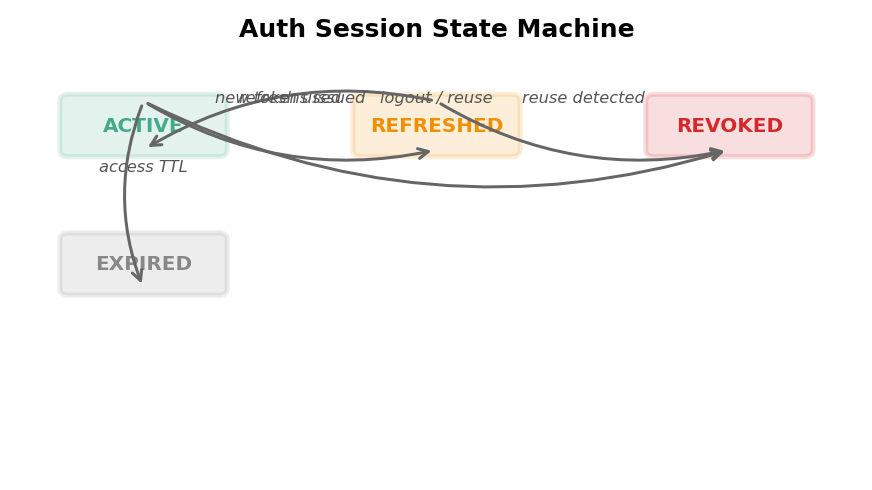
\includegraphics[width=0.65\textwidth]{images/statemachines/auth_session_statemachine.png}
  \caption{Auth Session State Machine}
  \label{fig:auth-statemachine}
\end{figure}
